\begin{figure}[tb]
  \centering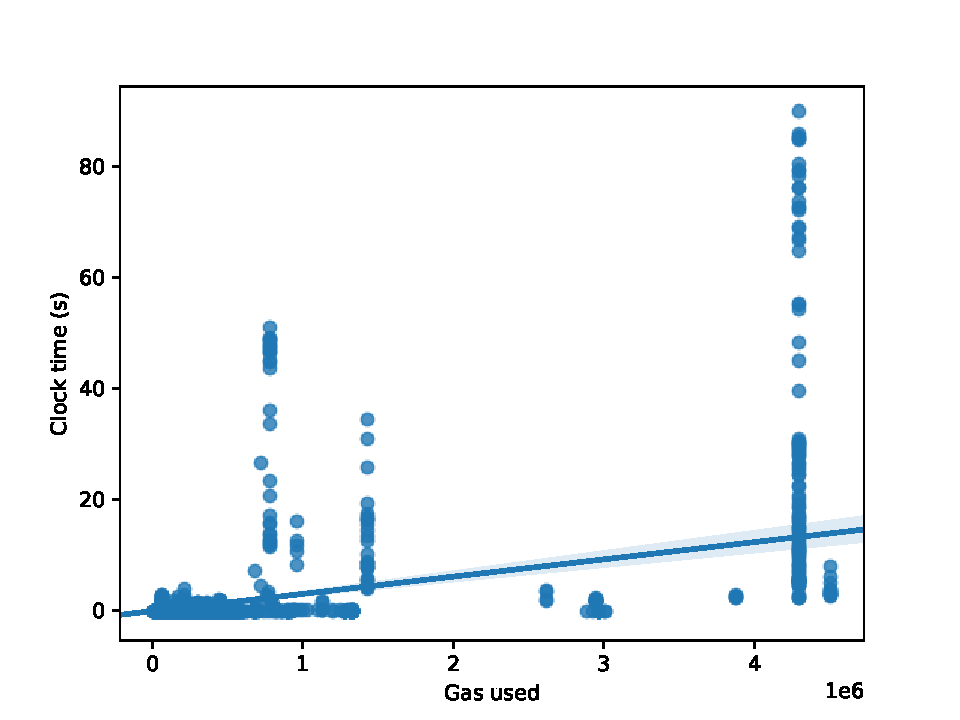
\includegraphics[width=\textwidth]{3-vm-security/figures/cpu-gas-extcodesize.pdf}
  \caption{Correlation between gas and clock time with DoS.}
  \label{fig:extcodesize-cpu}
\end{figure}

\section{Case Studies in Metering}
\label{sec:case-studies}

In this section, we instrument the C\texttt{++} client of the Ethereum blockchain, called \textit{aleth}~\cite{aleth}, and report some interesting observations about gas dynamics in practice.

\subsection{Experimental setup}
\point{Hardware} We run all of the experiments on a Google Cloud Platform (GCP)~\cite{gcp-compute-engine} instance with~4 cores~(8 threads) Intel Xeon at~2.20GHz,~8~GB of RAM and an SSD with a~400MB/s throughput.
The machine runs Ubuntu 18.04 with the Linux kernel version~4.15.0. We selected this hardware because it is representative of what has been reported as sufficient to run a full Ethereum node~\cite{node-incentive,pantheon-system-requirements,eth-hardware-requirements}.

\point{Software} To measure the speed of different instructions, we fork the Ethereum C\texttt{++} client, \textit{aleth}.
Our fork integrates the changes to the upstream repository until Jun-26 2019.
We choose the C\texttt{++} client for two reasons: first, it is one of the two clients officially maintained by the Ethereum Foundation~\cite{ethereum-foundation-github} with geth~\cite{geth}; second, it is the only of the two without runtime or garbage collection, which makes measuring metrics such as memory usage more reliable.

We add compile options to the original C\texttt{++} client to allow enabling particular measurements such as CPU or memory. Our measurement framework is open-sourced\footnote{\url{https://github.com/danhper/aleth/tree/measure-gas}} and available under the same license as the rest of \textit{aleth}.

\point{Measurements}
For all our measurements, we only take into account the execution of the smart contracts and ignore the time taken in networking or other parts of the software. We use a nanosecond precision clock to measure time and measure both the time taken to execute a single smart contract and the time to execute a single instruction. To measure the memory usage of a single transaction, we override globally the \lstinline[language=C++]{new} and \lstinline[language=C++]{delete} operators and record all allocations and deallocations performed by the EVM execution within each transaction. We ensure that this is the only way used by the EVM to perform memory allocation.

Given the relatively large amount of time it takes to re-execute the blockchain, we only execute each measurement once when re-executing. We ensure that we always have enough data points, where enough in the order of millions or more, so that some occasional imprecision in the measurements, which are inevitable in such experiments, do not skew the data.

In this section, the measurements are run between block \empirical{5,171,468 (Feb-28-2018)} and block \empirical{5,587,480 (May-10-2018)}, except in \autoref{ssec:system-resources} where we want to compare after and before EIP-150.

\begin{figure}[tb]
  \begin{subfigure}[t]{\columnwidth}
    \centering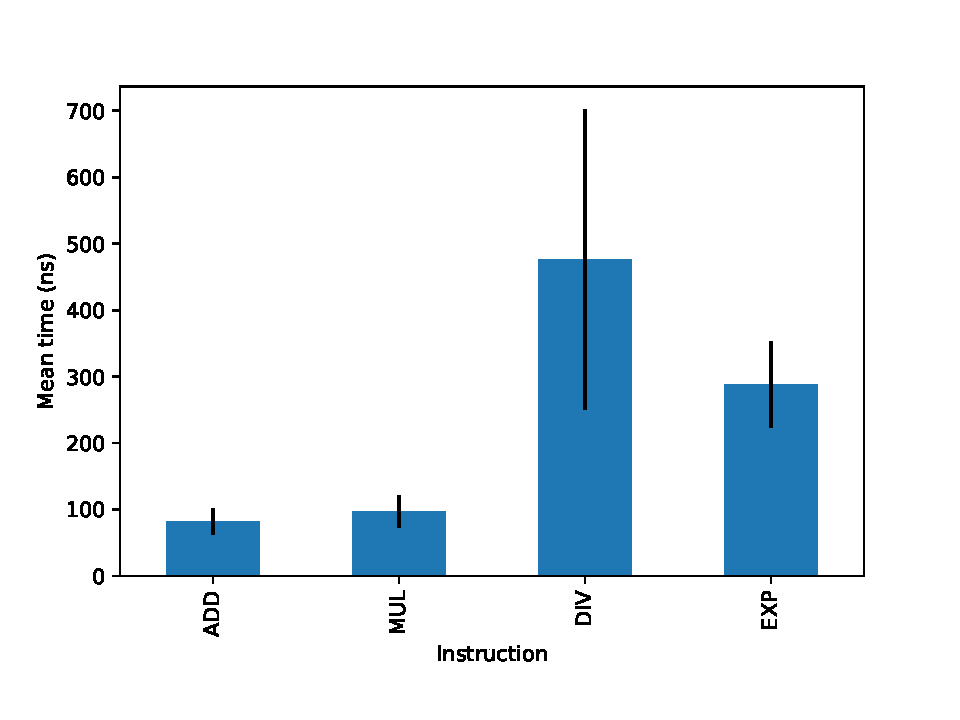
\includegraphics[width=\columnwidth]{3-vm-security/figures/arithmetic-microbench.pdf}
    \vskip -5mm
    \caption{Mean time for arithmetic instructions.}
    \vskip 5mm
    \label{fig:arithmetic-instruction-times}
  \end{subfigure}
  \begin{subfigure}[t]{\columnwidth}
    \centering
    \begin{tabular}{crrrr}
      \toprule
      \bf \multirow{2}{*}{Instruction} & \bf Gas            & \bf \multirow{2}{*}{Count} & \multicolumn{1}{c}{\bf Mean} & \bf Throughput \\
                                       & \bf cost           &                            & \textbf{time} (ns)           & (gas / $\mu$s) \\
      \midrule
      \texttt{ADD}                     & 3                  & 453,069                    & 82.20                        & 36.50          \\
      \texttt{MUL}                     & 5                  & 62,818                     & 96.96                        & 51.57          \\
      \texttt{DIV}                     & 5                  & 107,972                    & 476.23                       & 10.50          \\
      \texttt{EXP}                     & \textasciitilde 51 & 186,004                    & 287.93                       & 177.1          \\
      \bottomrule
    \end{tabular}
    \caption{Execution time and gas usage for arithmetic instructions.}
    \label{tab:arithmetic-instruction-times}
  \end{subfigure}
  \caption{Comparing execution time and gas usage of arithmetic instructions.}
\end{figure}

\subsection{Arithmetic Instructions}
In this experiment, we evaluate the correlation between gas cost and the execution time for simple instructions which include absolutely no IO access. We use simple arithmetic instructions for measurements, in particular the \lstinline{ADD}, \lstinline{MUL}, \lstinline{DIV} and \lstinline{EXP} instructions.

In \autoref{fig:arithmetic-instruction-times}, we show the mean time of execution for these instructions, including the standard deviation for each measurement.
We contrast these results with the gas cost of the different instructions in \autoref{tab:arithmetic-instruction-times}.
\lstinline{EXP} is the only of these instructions with a variable cost depending on its arguments --- the value of the exponent. We use the average gas cost in our measurements to compute the throughput.
We see that although in practice \lstinline{ADD} and \lstinline{MUL} have similar execution time, the gas cost of \lstinline{MUL} is~65\% higher than the gas cost for \lstinline{ADD}.
On the other hand, \lstinline{DIV}, which costs the same amount of gas as \lstinline{MUL}, is around~\emph{5 times slower} on average. \lstinline{EXP} costs on average \emph{10 times} the price of \lstinline{DIV} but executes~40\% faster.
Another point to note here is that \lstinline{DIV} has a standard deviation much higher than the other three instructions.
Although we were expecting that for such simple instructions, the execution time would reflect the gas cost, this does not appear to be the case in practice.
We will show in the coming sections that IO-related operations tend to make things worse in this regard.


\begin{table}[tb]
  \centering
  \setlength{\tabcolsep}{14pt}
  \caption{Correlation scores between gas and system resources.}
  \label{tab:correlation-scores}
  \begin{tabular}{clr}
    \toprule
    \thead[l]{Phase}              & \thead[l]{Resource} & \thead[r]{Pearson \\score}\\
    \midrule
    \multirow{4}{*}{Pre EIP-150}  & Memory              & 0.545             \\
                                  & CPU                 & 0.528             \\
                                  & Storage             & 0.775             \\
                                  & Storage/Memory      & \textbf{0.845}    \\
                                  & Storage/Memory/CPU  & 0.759             \\
    \midrule
    \multirow{4}{*}{Post EIP-150} & Memory              & 0.755             \\
                                  & CPU                 & 0.507             \\
                                  & Storage             & 0.907             \\
                                  & Storage/Memory      & \textbf{0.938}    \\
                                  & Storage/Memory/CPU  & 0.893             \\
    \bottomrule
  \end{tabular}
\end{table}

\subsection{Gas and System Resources Consumption}
\label{ssec:system-resources}
In this section, we analyse the gas consumption of Ethereum smart contracts and try to correlate it with different system resources, such as memory, CPU and storage.
As described in \autoref{sec:background}, EIP-150 influenced the price of many storage-related operations, which affected the gas cost of transactions. Therefore, we use a different set of transactions than for other case studies. We arbitrarily use block~\empirical{1,400,000} to block ~\empirical{1,500,000} for measurements before EIP-150 and block ~\empirical{2,500,000} to~\empirical{2,600,000} for measurements after EIP-150. We assume that the sample of~\empirical{100,000} blocks, which roughly corresponds to two weeks, is large enough to obtain reliable data.

We use our modified Ethereum client to perform the different measurements. To measure memory, we compute the difference between the total amount of memory allocated and the total amount of memory deallocated.
For CPU, we use clock time measurements as a proxy for CPU usage. Finally, for storage usage, we count the number of EVM words~(256 bits) of storage newly allocated per transaction.

We compute the Pearson correlation coefficient\footnote{Pearson score of 1 means perfect positive correlation, 0 means no correlation}~\cite{boslaugh2012statistics} between the different resources and the gas usage.
We also compute multi-variate correlations between gas consumption and multiple resources.
To compute the multi-variate correlation between multiple resources and gas usage, we first normalise the measurement vector of each targeted resource to have a mean of $0$ and a standard deviation of $1$.
Then, we stack the vectors to obtain a matrix of $m$ resources and $n$ measurements and transform it into a single vector of $n$ measurements using a principal component analysis~\cite{abdi2010principal}.
The vector we obtain represents the aggregated usage of the different resources and can be correlated with the gas usage.

We present our results in \autoref{tab:correlation-scores}.
A first observation is that EIP-150 clearly emphasises the domination of storage in the price of contracts.
We can see that storage alone has an extremely high correlation score, with a score of~\empirical{0.907} after EIP-150.
Memory usage is not as correlated as storage, but when combining both, they have the highest correlation score of~\empirical{0.938}.
Finally, an important point is that CPU time seems completely uncorrelated with gas usage.
Although it seems natural that CPU time by itself has a low correlation, as the gas cost is dominated by storage cost, adding the CPU time in the multi-variate correlation reduces the correlation.
It is not enough to make any conclusion yet but gives a hint that as long as the storage is not explicitly touched, it could be possible for contracts to be both cheap and long to execute.

\subsection{High-Variance Instructions in the EVM}
Here, we look at instructions which have a high variance in their execution time.
We summarise the instructions which had the highest variance in \autoref{tab:high-variance-instructions}.
There are two main reasons why the execution time may vastly vary for the execution of the same instruction.
First, many instructions take parameters.
Depending on these, the time it takes to run the particular instructions can vary wildly.
This is the case for an instruction such as \lstinline{EXTCODECOPY}.
The second reason is much more problematic and comes from the fact that some instructions may require to perform some IO access, which can be influenced by many different factors such as caching, either at the OS or at the application level.
The instruction with the highest variance was \lstinline{BLOCKHASH}.
\lstinline{BLOCKHASH} allows to retrieve the hash of a block and allows to look up to~256 block before the current one.
When it does so, depending on the implementation and the state of the cache, the EVM may need to perform an IO access when executing this instruction, which can result in vastly different execution times.
The cost of \lstinline{BLOCKHASH} being currently fixed and relatively cheap,~20 gas, it results in an instruction which is vastly under-priced. It is worth noting that in the particular case of \lstinline{BLOCKHASH}, the issue has already been raised more than two years ago in EIP-210~\cite{eip-blockhash}.
It discussed changing the price of \lstinline{BLOCKHASH} to~800 gas but at the time of writing the proposal is still in draft status and was not included in the Constantinople fork\footnote{Hard fork which took place on Feb 28 2019 on the Ethereum main network}~\cite{constantinople} as it was originally planned to be.

\begin{table}[tb]
  \centering
  \caption{Instructions with the highest execution time variance.}
  \label{tab:high-variance-instructions}
  \setlength{\tabcolsep}{3pt}
  \begin{tabular}{lrrr}
    \toprule
    \textbf{Instruction} & \textbf{Mean}          & \textbf{Standard}  & \textbf{Measurements} \\
                         & \textbf{time} ($\mu$s) & \textbf{deviation} & \textbf{count}        \\
    \midrule
    \texttt{BLOCKHASH}   & 768                    & 578                & 240,000               \\
    \texttt{BALANCE}     & 762                    & 449                & 8,625,000             \\
    \texttt{SLOAD}       & 514                    & 402                & 148,687,000           \\
    \texttt{EXTCODECOPY} & 403                    & 361                & 23,000                \\
    \texttt{EXTCODESIZE} & 221                    & 245                & 16,834,000            \\
    \bottomrule
  \end{tabular}
\end{table}

% \subsection{Branch Prediction and EVM Costs}

\begin{figure}[tb]
  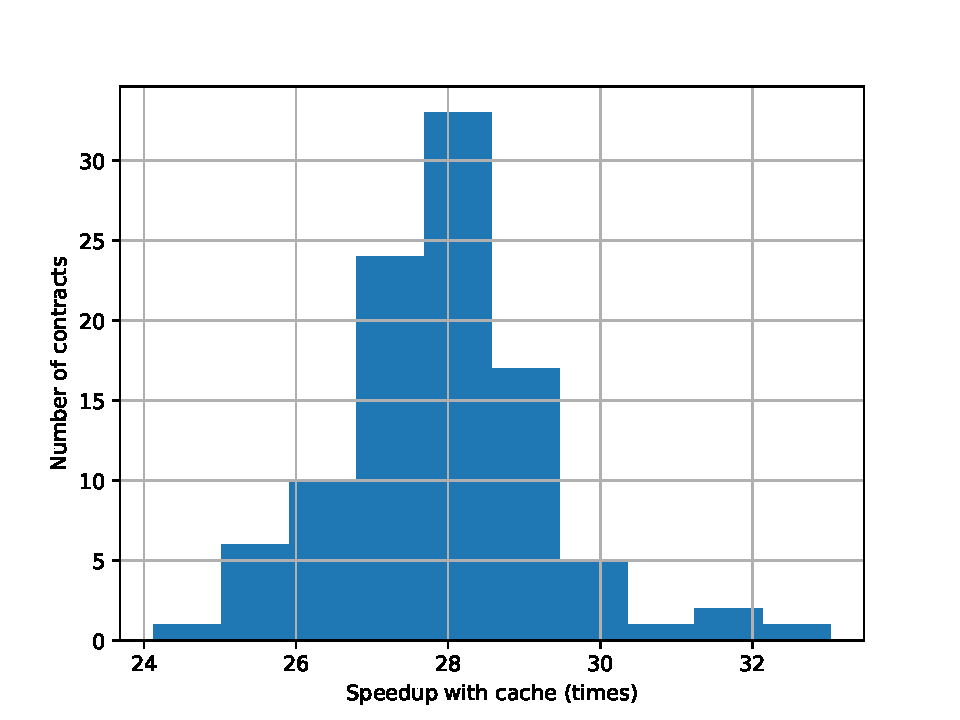
\includegraphics[width=\columnwidth]{3-vm-security/figures/cache-speed.pdf}
  \caption{Comparing throughput with and without page cache: $x$ axis is the relative speed improvement and $y$ axis is the number of contracts.}
  \label{fig:cache-measurement}
\end{figure}

\begin{figure}[tb]
  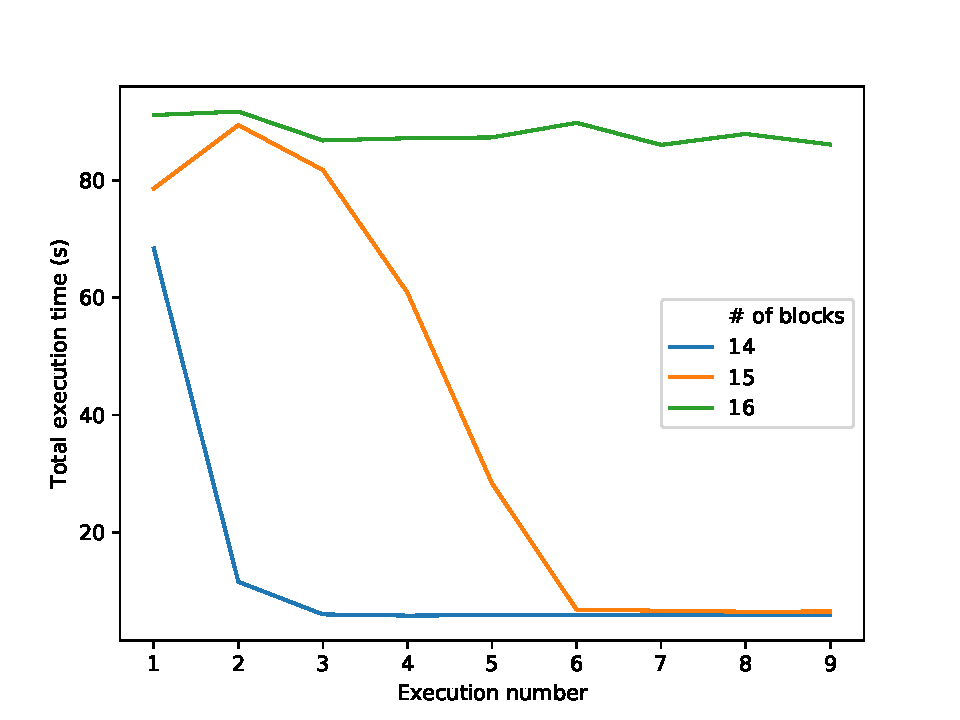
\includegraphics[width=\columnwidth]{3-vm-security/figures/cache-persistence.pdf}
  \caption{Measuring block execution speed with and without the effect of cache.}
  \label{fig:cache-persistence}
\end{figure}

\subsection{Memory Caches and EVM Costs}
\label{ssec:memory-caches}
Given the high variance in execution time for some instructions, we evaluate the effects caching may have on EVM execution speed. In particular, we evaluate both the speedup provided by the operating system page cache and the speedup across blocks provided by LevelDB LRU cache~\cite{leveldb-cache}. In these experiments, we fix the block number at height~\empirical{5,587,480}.

\point{Page cache} First, we evaluate how the operating system page cache influences the execution time by reducing the IO latency. We perform the experiment as follows:

\begin{enumerate}
  \item Generate a contract
  \item Run the code of the contract $n$ times
  \item Run the code of the contract $n$ times but drop the page cache between each run
\end{enumerate}
%
We perform this for~\empirical{100} different contracts and measure the execution time for the versions with and without cache. We generate relatively large contracts, which consume on average~\empirical{800,000} gas each.
Although the method is somewhat crude, it provides a good approximation of the extent to which the state of the page cache influences the execution time of a contract.
In \autoref{fig:cache-measurement}, we show a distribution of the contracts throughput in terms of gas per second, with and without cache. We see that contracts execute between~\empirical{24} and~\empirical{33} times faster when using the page cache, with more than half of the contracts executing between~\empirical{27} and~\empirical{29} times faster.
This vast difference in the execution speed is due to IO operations, which use LevelDB~\cite{ghemawat2011leveldb}, a key-value store database, under the hood. LevelDB keeps only a small part of its data in memory and therefore needs to perform disk access when the data was not found in memory.
If the required part of the data was already in the page cache, no disk access will be required.
When keeping the page cache, all the items seen by the contract recently will already be available in the cache, eliminating the need for any disk access. On the other hand, if the caches are dropped, many IO-related operations will result in disk access, which explains the speedup.
We notice that in the contracts with the highest speedup, \lstinline{BLOCKHASH}, \lstinline{BALANCE} and \lstinline{SLOAD} are in the most frequent instructions.
It is worth noting that if the generated contracts are small enough, most of the data will be in memory and dropping the page cache will have much less effect on the runtime.
Indeed, when running the same experiment with contracts consuming on average~\empirical{100,000} gas, only a 2 times average speedup has been observed.
%
\point{Caching across blocks} In the next experiment, instead of measuring the cache impact by running a single contract multiple times, we evaluate how the cache impacts the execution time across blocks. In particular, we measure how many blocks need to be executed before the data cached during the previous execution of a contract gets evicted from the different caches. To do so, we perform the following experiment.

\begin{enumerate}
  \item Generate $n$ blocks, with different contracts in each
  \item Execute sequentially all the blocks and measure the execution time
  \item Repeat the previous step $m$ times in the same process and record how the execution speed evolves
\end{enumerate}

We set $m$ to 10 and we try different values for $n$ to see how many blocks are needed for the cache not to provide any further speedup.
We use the first execution to warm up the node and use the $9$ other executions for our measurements.
We find that in our setup, assuming the blocks are full (i.e. close to the gas limit in terms of gas), $16$ blocks are enough for the cache not to provide any more speedup.
We plot the results for \empirical{$n = 14$}, \empirical{$n = 15$} and \empirical{$n = 16$} in \autoref{fig:cache-persistence}.
When \empirical{$n = 14$}, we see that the second execution is much faster than the first one and that after the third execution, the execution time stabilises at around \empirical{6s} to execute the \empirical{$14$} blocks. For \empirical{$n = 15$}, the execution time takes longer to decrease, but eventually also stabilises around the same value. It is slightly higher than when \empirical{$n = 14$} because it has one more block to execute.
However, once we reach \empirical{$n = 16$}, we see that the execution time hardly decreases and stays stable at around \empirical{85s}. We conclude that at this point, almost nothing that was cached during the previous execution of the block is still cached when re-executing the block.

This means that if a deployed contract function were re-executed more than 16 blocks after its initial execution, it would execute as slowly as the first time.
This shows that not only the cache has a very high impact on execution time but also that the cached information is evicted relatively quickly.

\subsection{Summary}
In this section, we empirically analysed the gas cost and resource consumption of different instructions. To summarise:
\begin{itemize}
  \item We see that even for simple instructions, the gas cost is not always consistent with resource usage. Indeed, even for instruction with very predictable speed, such as arithmetic operations, we observe that some instructions have a throughput~\empirical{5} times slower than others.
  \item We notice that while most instructions have a relatively consistent execution speed, other instructions have large variations in the time it takes to execute. We find that these instructions involve some sort of IO operation.
  \item Finally, we demonstrate the effect that the page cache has on the execution speed of smart contracts and then show the typical number of blocks for which the page cache still provides speed up.
  \item Overall, we see that beyond some pricing issues, the metering scheme used by EVM does not allow to express the complexity inherent to IO operations.
\end{itemize}
